\documentclass[a4paper, 11pt, onepage]{scrreprt}

\usepackage{fontspec}
\setmainfont{Linux Libertine O}
\usepackage{polyglossia}
\usepackage{amssymb}
\usepackage{amsmath}
\usepackage{mathtools}
\usepackage{bbold}
\usepackage[hyperref]{xcolor}
\usepackage{graphicx}
\usepackage{listings}
\usepackage{caption}
\usepackage{wrapfig}
\usepackage{float}
\usepackage{tabularx}
\usepackage{booktabs}
\usepackage{numprint}
\usepackage{hyperref}

\newcommand\wiki{\textsc{Wikipedia}}
\newcommand\ew{\textsc{English Wikipedia}}
\newcommand\sew{\textsc{Simple English Wikipedia}}
\newcommand\tableref[1]{\hyperref[#1]{Table \ref*{#1}}}
\newcommand\figureref[1]{\hyperref[#1]{Figure \ref*{#1}}}
\newcommand\sectionref[1]{\hyperref[#1]{Section \ref*{#1}}}
\newcommand\maps[1]{\xrightarrow{\mathcal{#1}}}
\newcommand\card[1]{\lvert #1 \rvert}
\newcommand\suchthat{\, \middle| \,}
\newcommand\given{\, \middle| \,}
\newcommand\proba[2][]{P_{#1} \left( #2 \right)}

\DeclareMathOperator*{\argmin}{\arg\,\min}
\DeclareMathOperator*{\argmax}{\arg\,\max}

\renewcommand\chaptername{Section}
\renewcommand\thechapter{\Roman{chapter}}

\DeclareGraphicsExtensions{.png, .jpeg, .jpg, .svg, .eps}
\graphicspath{{./img/}}

\hypersetup{
  colorlinks = true,
  linkcolor = violet,
  urlcolor = teal,
  citecolor = gray
}

\begin{document}
\begin{titlepage}
  \begin{center}
    \noindent\rule{\textwidth}{0.4pt}
    {\huge\bfseries Improving text readability using\\
      \sew\\}
    \noindent\rule{\textwidth}{0.4pt}\\
    % ----------------------------------------------------------------
    \vspace{1.5cm}
    {\large
    \begin{tabularx}{\textwidth}{lXll}
      \textbf{Author:} & \textsc{Hugo Mougard} &
      \textbf{Director:} & \textsc{Akiko Aizawa} \\
      \textbf{Tutor:} & \textsc{Colin de la Higuera} &
      \textbf{Advisor:} & \textsc{Pascual Martínez-Gomez} \\
    \end{tabularx}}\\[5pt]
    % ----------------------------------------------------------------
    \vfill
    \parbox{0pt}{\large \begin{tabbing}
        \textbf{Sending institution:} \= National Institute of Informatics \kill
        \textbf{Sending institution:} \> \textsc{Université de Nantes, France} \\
        \textbf{Hosting institution:} \> \textsc{National Institute of
        Informatics, Japan} \\
      \end{tabbing}}
    \vfill
    {\LARGE ATAL Master 2 internship report}
    \vfill
    % ----------------------------------------------------------------
    
\includegraphics[width=0.16\textwidth]{img/nii.png}
    \hfill
    \hfill
    
\includegraphics[width=0.19\textwidth]{img/lina.png}
    \hfill
    
\includegraphics[width=0.19\textwidth]{img/univ.eps}
    \vfill
    {July 2014}
  \end{center}
\end{titlepage}

\tableofcontents

\chapter{Acknowledgments}

I would like to thank Aizawa-sensei and Katsu-san for their precious
help before our arrival to Japan, and their support during our stay.

I also wouldn't have been able to conduct this internship without the
scientific advising of Aizawa-sensei and Pascual-san, I thank them for
all their good insight, even though I am convinced I didn't make the
best of it.

It was also very nice to have someone exterior to discuss ideas with
when I wanted to, I thank Colin de la Higuera for that.

Finally I would like to thank Fujinuma-san for being so nice with me
during the internship and for showing me so many things, ranging from
Japanese culture to scientific projects.

\chapter{Laboratory presentation}

\section{National Institute of Informatics}
\label{sec:national-institute-of-informatics}

This internship is taking place at the National Institute of
Informatics in Tokyo, Japan.

\section{Aizawa Laboratory}
\label{sec:aizawa-laboratory}

The team that welcomed me for this work is Aizawa Laboratory. It is
led by Professor Akiko Aizawa. At the time of this writing, the
laboratory has 18 members and strong partnerships with ex-members of
the laboratory.

Its expertise lies in several sub-domains of NLP: gaze-NLP, Analysis
and mining of scientific papers, mathematical information retrieval,
etc.

The work presented in this report has been done in the gaze-NLP
work group. It is so despite the fact that finally no gaze information
was used in the developed approach, because readability has very
strong connections with gaze NLP research.

\chapter{Introduction}

Whether it is to teach children how to read or to assess the
comprehensiveness of technical manuals, readability has been studied
for around two centuries for its impact in both engineering and
scientific endeavors.

Despite this interest of the scientific community, the approaches
proposed have for a long time focused on simple readability
formulas. It is only in recent years that scientists have been able to
come up with more interesting methods, leveraging both the speed of
modern computers and the unparalleled amount of data available on the
internet.

The focus of this internship is to improve on those methods. To be
more specific, most methods consider documents as a whole when
analyzing their readability, which makes it hard for users to
understand which parts are the most important to rework. We aim at
providing a fine-grained analysis of readability in this work. In the
same way than the recursive approach to sentiment analysis
\cite{socher2013recursive} allows users to detect which parts of a
sentence convey which sentiment, we aim at detecting which parts of a
sentence are readable or non readable, and for which reasons.

\chapter{Prior art}
\label{sec:sota}

\section{Early works and readability formulas}
\label{sec:early-works-and-formulas}
Readability has been studied extensively. The first works in this area
date back to more than a century ago: in 1893, Sherman published a
book \cite{sherman1893analytics} where he compared modern English and
English spoken four centuries before with considerations that are very
alike the ones that current readability studies outline. Then, in
1921, Thorndike computed a list of ten thousand easy-to-read words
\cite{thorndike1921teacher}. This list got used shortly thereafter by
teachers trying to select good books for children learning to read
\cite{lively1923method}: they went through the process of estimating
the readability of many books thanks to a basic formula and
Thorndike's list.

This was the beginning of an important branch of research focusing on
how to best estimate the readability of a text thanks to simple
formulas. Among the most famous methods, it is interesting to mention
the Flesch Reading Ease \cite{flesch1948new} which introduced the use
of a combination of the average number of words per sentence and the
average number of syllables per word to estimate the readability of a
text, because most of the subsequent approaches also use those
metrics. This method yields a 0.91 correlation with text understanding
and has been used outside of research to improve the readability of a
vast amount of publications, yielding excellent results in readership
increase.

Roughly at the same time, Dale and Chall introduced a readability
formula that uses a list a words instead of the average number of
syllables per word to estimate readability
\cite{dale1948formula}. This more precise definition of world
difficulty allows this metric to reach a 0.93 correlation with text
understanding and because of that has been one of the most used
formulas in research.

Later works brought formulas that are easier to compute or give
slightly better results. Some also give their result as the grade that
would be required to be able to read the input text. Overall are all
using the same variables as either Flesch or Dale and Chall
\cite{mclaughlin1969smog, kincaid1975derivation,
  chall1995readability}.

Despite their useful applications, readability formulas are not
perfect. Some works have detailed their problems convincingly
\cite{duffy1985readability, schriver2000readability}. Among the most
important problems is using sentence length to model syntactic
complexity: of the following sentences, (1.) is often considered
easier to understand than (2.), despite being lengthier:
\begin{enumerate}
\item The mouse ate the cheese, and then the rat ate the mouse, and
  after that, the cat ate the rat and died.
\item The cat that ate the rat that ate the mouse that ate the cheese
  died.
\end{enumerate}
Another important problem is modeling word complexity by word length,
which doesn't consider the fact that affixes are known to readers, so
very long words can be simple, and some short words are, in contrary,
relatively not known: curr (to make a murmuring sound), is not well
known, while reinventing is actually easy to understand for most early
readers because re- and -ing are commun affixes and invent is well
known.

Finally, the fact that many formulas only consider short windows of a
text to estimate its readability make them not reliable without
repetition of the measure at several points in a text and an averaging
(which is what Dale \& Chall does by default).

To address those shortcomings, scientists have recently proposed
machine learning based approaches. The next section details those
works.

\section{Machine Learning approaches}
\label{sec:ml-approaches}

More recently, from 2006 onwards, \sew has been rightly seen as an
important resource for readability studies. Many scientists have used
it to compute parallel corpora of readable their hard-to-read
counterparts sentences.

\section{Readability research using \wiki}
\label{sec:wiki-approaches}

\chapter{Work}
\label{cha:work}

To address the lack of corpora and tooling in the readability domain,
we propose a method to easily build a parallel corpus using \sew's
revision history. This approach is not novel, since 2008, researchers
have used \sew's revision history to great effect
\cite{nelken2008mining}. What is novel is that we plan on releasing
the corpus with a permissive license and associated tooling to reduce
the entry cost of readability research and allow comparison between
methods on a level ground.

To be able to correctly investigate fine-grained readability, we
propose a software suite to represent results of readability system in
a way that suits analysis.

Finally we experiment with lexical re-writings using our system.

Details on those three main axes follow.

\section{Automatic readability parallel corpus creation}
\label{sec:corpus}

Most machine learning approaches efficiencies are directly dependent
on the amount of data at their disposal. Those approaches are used in
more scientific domains every day for their effectiveness. This is
what led people to describe data efficiency as “unreasonable”
\cite{halevy2009unreasonable}. In this context, it seems that being
able to gather automatically data is of utmost importance. Moreover,
raw data is often not enough. Most techniques require a lengthy and
costly annotation process. For this reason, researchers in every
domain using machine learning invest time finding clever techniques to
automatically obtain annotated corpora.

In readability, such a clever technique is to leverage the power of
\wiki, and in particular \sew. To do so, mainly two techniques have
been used: the first is to use the articles present both in the
regular \ew{} and in \sew{} and use their comparison as a starting
point to build a parallel corpus. This approach has been used with
great success in \cite{zhu-bernhard-gurevych:2010:PAPERS} and has
resulted in the
PWKP-108016\footnote{\url{https://www.ukp.tu-darmstadt.de/data/sentence-simplification/simple-complex-sentence-pairs/}}
dataset.The second is to use the revision history of \sew, as
showcased in \cite{yatskar2010sake}. In this work we use the second
approach.

The main rationale behind not using the existing PWKP-108016 corpus
and instead making one of our own is that we believe the technique
used to automatically construct the corpus from a revision history is
a general process and can therefore be extended to many data sources
beyond \wiki. Those possible extensions include many of the processes
of the professional publishing world. If shown to be efficient, big
corpora could be gathered from journalists, writers, scientists, etc.
In contrary, it has been shown to be extremely hard to find good
comparable corpora outside of \wiki{} and some restricted institution
publications such as the European Parliament \cite{koehn2005europarl},
which makes the first approach hard to generalize. Finally, the
outputs made public by \cite{yatskar2010sake} are of high quality but
limited in quantity and do not incorporate some important features
such that the original sentence from which pairs were extracted, nor
does this release include any code to manipulate the files.

To build automatically our corpus, we leverage the fact that when
editing \sew, contributors have the possibility to write a commit
message, so that other people can quickly browse history and guess the
role of a particular commit. This allows us to automatically detect if
a particular commit was intended to fix a readability issue or was
serving another purpose (improving the content of the article,
cleaning the wiki, vandalizing, …). This usage of metadata is not
novel, it was used in the \textsc{Simpl} approach presented in
\cite{yatskar2010sake}. Though, we fine-tune the heuristic used to
address some problems encountered in this article and to harden the
process. An example of readability edit can be seen in
\figureref{fig:dan-kelly}.

\begin{figure}[H]
  \centering
  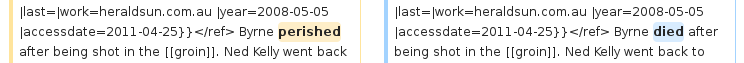
\includegraphics[width=\textwidth]{dan-kelly}
  \caption{An edit of the Dan Kelly article with the commit message
    “use simple english here”}
  \label{fig:dan-kelly}
\end{figure}

The heuristic we use to gather edits is extremely simple: once
stripped of the category information, we only consider edits with
commit messages $m$ so that:

\[
m \in \left\{\text{“simplify”}, \text{“simplifying”},
  \text{“simplified”}, \text{“simplification”},
  \text{“simpler”}\right\}
\]

This may seem drastic but we believe it is necessary due to the many
noisy commits introduced with broader rules. To illustrate this point,
we can consider the commit messages of
\tableref{tab:problematic-commits}. We can see that commit \#1 has two
purposes, one of which will bring noise (the wikification). Commit \#2
contains one of the matching terms, but we should not consider
it. It's not clear if commit \#3 tries to address readability or not.

\begin{table}[H]
  \centering
  \caption{Problematic commit messages}
  \begin{tabular}{rp{12cm}}
    \toprule
    \# & Commit message \\
    \midrule
    1 & “simplified, and wikified” \\
    \addlinespace
    2 & “wikify. needs simplifying” \\
    \addlinespace
    3 & “exhaustive, to help us work out titles of articles - lots of
    discussion here, and no, this is not simple engouh yet” \\
  \end{tabular}
  \label{tab:problematic-commits}
\end{table}

Furthermore, we determined by an empirical study that those commits
represented an important part of the commits we might have retrieved
with a broader rule, so we simply did not consider them.

The next step for the creation of the corpus is to compute the precise
edit that the contributor made. To do so, we tokenize and sentence
split both the original version of the article and its revision using
OpenNLP\footnote{\url{https://opennlp.apache.org/}}. Then, we use
Myers' alignment algorithm \cite{myers1988optimal} to compute optimal
alignments at the world and sentence levels. We rely on the
implementation proposed by
jgit\footnote{\url{http://www.eclipse.org/jgit/}}.

The goal being to obtain a re-usable corpus, we propose the complete
pipeline on
github\footnote{\url{https://github.com/m09/readability}}. It is
freely re-usable.

The obtained corpus has important noise problems. A quick glance at
\tableref{tab:problematic-edits} is sufficient to understand that some
edits are not readability edits, but either alignment deficiencies or
edits serving complementary roles. When filtered to only consider
revisions of 5 words at most, to match the policy used in
\cite{yatskar2010sake}, the number of entries is reduced to
\numprint{23507}.

\begin{table}[H]
  \centering
  \caption{Problematic edits}
  \begin{tabular}{rp{6cm}p{6cm}}
    \toprule
    \# & Original version & Revised version \\
    \midrule
    1 & , and & . she also used them in her arguments about \\
    \addlinespace
    2 & 2010 federal election, is russell matheson, a member & size\\
  \end{tabular}
  \label{tab:problematic-edits}
\end{table}

unfiltered corpus has \numprint{43753} entries. However,
it has important noise problems. A quick glance at
\tableref{tab:problematic-edits} is sufficient to understand that some
edits are not readability edits, but either alignment deficiencies or
edits serving complementary roles. When filtered to only consider
revisions of 5 words at most, to match the policy used in
\cite{yatskar2010sake}, the number of entries is reduced to
\numprint{23507}.
The resulting resource is enriched with part-of-speech, and syntactic
parsing annotations and is proposed in an XML format to optimize
re-usability.

\section{Lexical enhancements}
\label{sec:lexical-enhancements}

With this corpus at our disposal, we next define a way to use it as a
lexical dictionary. The goal is to allow authors to pick simpler words
than the ones they used, in an efficient manner. In what follows, we
will denote multiset of all rewritings of $x$ in $y$ in $\mathcal{D}$
by $x \maps{D} y$ a,d we will use $\_$ as a joker to denote any word.

The first approach and the most basic one, given a dictionary
$\mathcal{D}$ and for a word $w$, is to propose as lexical rewriting
candidates the set $R_w$ such that:

\[
R_w = \left\{r \suchthat w \maps{D} r\right\}
\]

But obviously, while this approach will have a important recall, it
will be extremely noisy and will not be of any real help to an author,
the time lost cruising through the noise outweighing the benefits of
the correct lexical enhancements.

A first improvement is to use the part of speeches available in the
corpus to make sure they match. That will already somewhat reduce
lexical ambiguity. That allows us to refine the definition of $R_w$ as
follows, $p_w$ begin the part of speech of $w$:

\begin{equation*}
  R_w = \left\{
    r \suchthat u \maps{D} r \land u = w \land p_u = p_w
  \right\}
\end{equation*}

We then introduce scores, so that it becomes possible to distinguish
between good and bad lexical enhancements with a precise metric. To
ease further discussion, we now introduce some probabilities. The
probability of a mapping $w \maps{D} r$ is:

\begin{equation*}
  \proba{w \maps{D} r} = \frac{\card{w \maps{D} r}}{\card{\_ \maps{D} \_}}
\end{equation*}

The probability of $w \maps{D} r$ given $w \maps{D} \_$ is:

\begin{equation*}
  \proba{w \maps{D} r \given w \maps{D} \_} = \frac{\card{w \maps{D} r}}{\card{w \maps{D} \_}}
\end{equation*}

The first one, named $\mathcal{S}_{occ}$, is a log of the basic count
of occurrences of a precise lexical enhancement in our dictionary. We
define it in precise terms as:

\begin{equation*}
  \mathcal{S}_{occ}(w \maps{D} r) = \log \proba{w \maps{D} r}
\end{equation*}

This score is still too basic for our needs. Its main shortcoming is
that it outlines mainly punctuation and tool-words rewritings. Those
are mainly linked to syntax and can't be handled by a purely lexical
rewriting system at any acceptable level of performance. The following
scores try to fix this punctuation and tool-words focus to turn it
into a lexical focus.

To accomplish this shift, we define the quality of a rewriting of $w$
into $r$ as the probability of a human rewriting $w$ into $r$. To
approximate this quantity, we use a language model. By combining a
language model to the information we have in our corpus, it is
possible to derive a measure close to this probability. The language
model we used was trained at a bi-gram level but would have been
trained at a tri-gram level if it was not for the lack of memory of
the machine used.

The score $\mathcal{S}_{lm}$ is one way to capture the above
definition, with $\proba[lm]{w}$ the language model probability of
$w$:

\begin{equation*}
  \mathcal{S}_{lm}(w \maps{D} r) = \log \frac{\proba{w \maps{D} r}}%
  {\proba[lm]{w}}
\end{equation*}

Note that while this score has some nice properties regarding the
quality of rewritings we defined above, it is not the log of a
probability, which is not a problem to compare rewritings but might
very well be to use those rewritings in a broader framework, for
example when performing the automatic rewriting of a text, we will
later see how we cope with those issues.

\section{Automatic rewriting of texts}
\label{sec:rewriting}

To rewrite automatically texts, we use weighted finite-state
transducers that consider the scores defined
in \sectionref{sec:lexical-enhancements} as weights to rewrite any
input text.

We define a finite-state transducer over a semi-ring $(\mathbb{K},
\oplus, \otimes, \mathbb{0}, \mathbb{1})$ (that we will use to combine
the outputs of a score function) as an 8-tuple that follows the
definition given by \cite{mohri2004weighted}: $T = (\Sigma, \Delta, Q,
I, F, E, \lambda, \rho)$ where $\Sigma$ is the finite input alphabet
of the transducer; $\Delta$ is the finite output alphabet; $Q$ is a
finite set of states; $I \subseteq Q$ the set of initial states; $F
\subseteq Q$ the set of final states; $E \subseteq Q \times (\Sigma
\cup \{\varepsilon\}) \times (\Delta \cup \{\varepsilon\}) \times
\mathbb{K} \times Q$ a finite set of transitions; $λ : I \rightarrow
\mathbb{K}$ the initial weight function; and $ρ : F \rightarrow
\mathbb{K}$ the final weight function mapping $F$ to $\mathbb{K}$.

We construct such a transducer for a given input text of $n$ tokens
noted $t_1 \dots t_{n}$ as follows, where $\mathcal{T}$ is the set of
all tokens in written English, and $\mathcal{S} : \mathcal{D}
\rightarrow \mathbb{K}$ is the score we use, with its semi-ring
$(\mathbb{K}, \oplus, \otimes, \mathbb{0}, \mathbb{1})$ attached:

\begin{align*}
  \Sigma & = \mathcal{T} \\
  \Delta & = \mathcal{T} \\
  Q & = \left\{ q_i \suchthat 0 \leq i \leq n \right\} \\
  I & = \{ q_0 \} \\
  F & = \{ q_n \} \\
  E & = \left\{ (q_{i - 1}, t_i, r, s, q_i) \suchthat t_i
    \maps{D} r \land s = \mathcal{S}\left(\ t_i \maps{D} r \right)\right\} \\
  I & : x \mapsto \mathbb{1} \\
  F & : x \mapsto \mathbb{1} \\
\end{align*}

Now, we can define semi-rings to use with the constructed
transducer. We mainly consider two use-cases, each of them requiring a
different semi-ring:

\begin{figure}[H]
  \centering
  \begin{enumerate}
  \item from the transducer and an input text, calculate the top $n$
    transductions. This is the classical task we aim for in
    statistical machine translation;
  \item from the transducer and an input text, get an idea of how the
    system rewrites the text at a certain level of confidence.
  \end{enumerate}
  
  \caption{Use-cases of text rewriting}
\label{fig:use-cases}
\end{figure}

The motivation for the second use-case is maybe not clear at
first. The reason for its existence is that, even for a very long
text, a top 100 of the rewritings might very well return 100 different
single token modifications while we would want to see the complete
text rewritten at once at a certain level of confidence. The Negative
MiniMax semi-ring below allows us to obtain this threshold effect
while the Negative Log semi-ring allows us to compute precise tops,
and is the log equivalent of the $(\mathbb{R}, +, *, 0, 1)$ semi-ring
for probabilities.

\begin{table}[H]
  \centering
  \begin{tabular}{rccccc}
    \toprule
    Semiring & $\mathbb{K}$ & $\oplus$ & $\otimes$ & $\mathbb{0}$ & $\mathbb{1}$
    \\
    \midrule
    Negative Log & $\mathbb{R}^{-} \cup \{-\infty\}$ & $+_{\log}$ & $+$ & $-\infty$ & $0$ \\
    Negative MinMax & $\mathbb{R}^{-} \cup \{-\infty\}$ & $\min$ & $\max$ & 0 & $-\infty$ \\
  \end{tabular}
  \caption{Interesting semi-rings for $\mathcal{S}_{occ}$}
  \label{tab:semi-rings}
\end{table}

We can almost directly use those semi-rings with the
$\mathcal{S}_{lm}$ score function. But since it is not the log of a
probability, we don't have the guarantee that for any $w \maps{D} r$,
$\mathcal{S}_{lm}\left( w \maps{D} r \right) \in \left]-\infty,
  0\right]$. To fix this problem, we normalize all the scores
$\mathcal{S}_{lm}$ as follows:

\[
\mathcal{S}_{lmn} \left( w \maps{D} r \right)
= \mathcal{S}_{lm} \left( w \maps{D} r \right)
- \argmax_{w' \maps{D} r'} \mathcal{S}_{lm} \left(w' \maps{D} r' \right)
\]

The $\mathcal{S}_{lmn}$ function can be used with the semi-rings we
defined for $\mathcal{S}_{occ}$.

It is now possible to address the two use-cases mentioned in
\figureref{fig:use-cases} by using the Viterbi algorithm
\cite{forney1973viterbi} with Negative Log as semi-ring for the first
use-case and Negative MinMax for the second.

The next section details how we built a framework to get interesting
feedback on both the rewriting and the lexical enhancement
approaches.

\section{Fine-grained readability analysis framework}
\label{sec:framework}

Considering that automatic evaluation of readability rewriting and
lexical enhancement is a very hard task, we then focused on producing
a high quality testing environment to be able to quickly assess
manually the quality of an approach. It was also the occasion to
expose those results to other programs by creating a server that could
easily be used by any other tool-chain.

We used \href{http://www.playframework.com/}{Play Framework} and
\href{https://facebook.github.io/react/}{React} to create a web client
that satisfies the constraints exposed above. \figureref{fig:ui} shows
an example usage.

\begin{figure}[H]
  \centering
  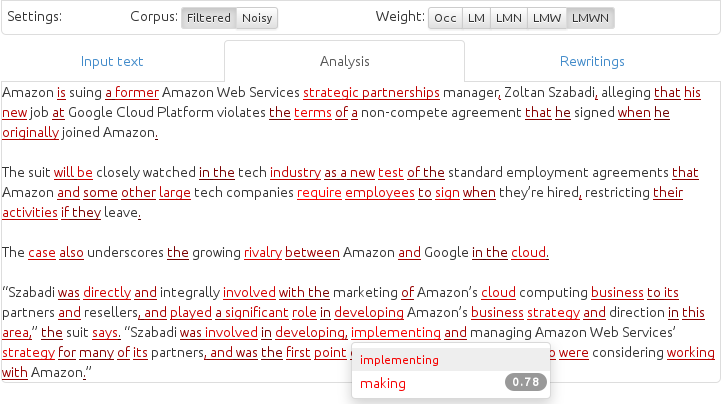
\includegraphics[width=\textwidth]{ui}
  \caption{\textsc{Readability Lab} interface}
  \label{fig:ui}
\end{figure}

\chapter{Open source contributions}
\label{cha:oss-contribs}

During this internship I had the opportunity to contribute to the open
source natural language processing community. What follows is a list
of those contributions.

\section{Enhancements of existing software}
\label{sec:enhancements}

\begin{itemize}
\item
  \href{https://bugs.eclipse.org/bugs/show_bug.cgi?id=433163}{Wikitext
    parser bug filing}
\item \href{https://issues.apache.org/jira/browse/OPENNLP-676}{OpenNLP
    POSTagger bug filing with patch}
\item \href{https://issues.apache.org/jira/browse/UIMA-3913}{uimaFIT
    enhancement proposal}
\end{itemize}

\section{uimaFIT components}
\label{sec:uimafit-components}

\begin{itemize}
\item sentence alignment analysis engine, using Myers' algorithm
\item word alignment analysis engine, using yet again Myers' algorithm
\item \href{https://berkeleylm.googlecode.com/}{BerkeleyLM} uimaFIT
  wrapper
\item readability formulas uimaFIT calculator
\end{itemize}

\section{Miscellaneous}
\label{sec:misc-software}
\begin{itemize}
\item Wikimedia PostgreSQL importer
\item Generic implementation of Aho-Corasick
\end{itemize}

\chapter{Conclusions  et perspectives}

\bibliographystyle{apalike2}
\bibliography{report.bib}

\end{document}
%%% Local Variables: 
%%% coding: utf-8
%%% mode: latex
%%% TeX-engine: xetex
%%% End: 
